\begin{problem}{能量球}{能量球.in}{能量球.out}{1 second}

在一个二维坐标里面,依次放入n个圆球,每个圆球可放在$x-y$轴的任意整数坐标内,现在定义一种判断放入的第$i$编号的圆球$(x_i,y_i)$是否是能量球的方法:如果不存在第$j$编号球$(x_j,y_j)$使得$x_j<x_i,y_j \leq y_i$或者$x_j \leq x_i,y_j<y_i$,那么就认为第$i$编号球是能量球。现在请你判断一下,在放入$n$个圆球之后,有多少颗能量球。
\begin{center}
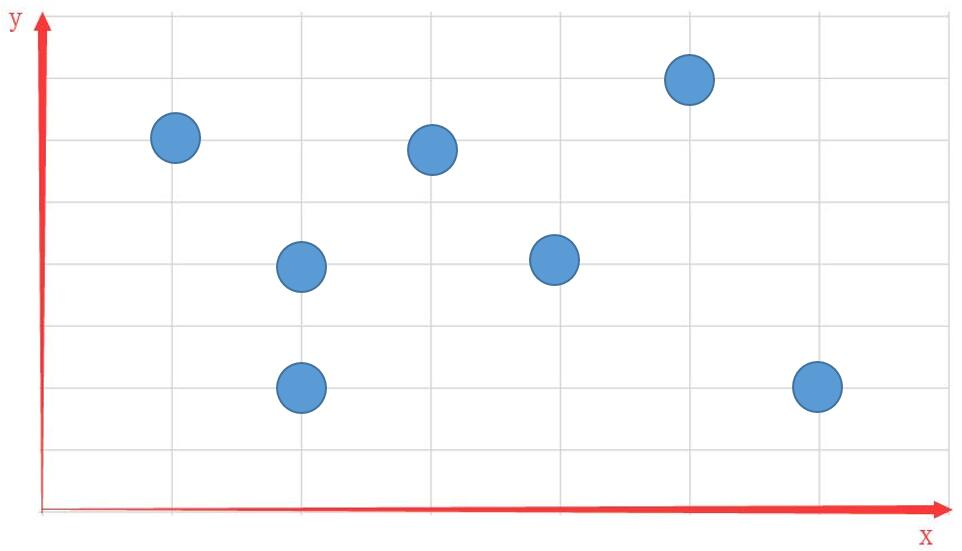
\includegraphics[width=0.4\textwidth]{pics/B.jpg}
\end{center}
\InputFile

第一行输入一个整数$n(1 \leq n \leq 10000)$

接下来$n$行每行输入两个整数$x_i$和$y_i$ $(1 \leq x_i,y_i \leq 10000)$表示放入的第$i$编号圆球的坐标

\OutputFile

输出有多少颗能量球$ans$

\Examples

\begin{example}
\exmp{
5
1 2
2 3
3 5
6 9
10 13
}{
1
}%
\exmp{
5
1 12
2 8
3 6
4 5
5 5
}{
4
}%
\end{example}
\textbf{注意:圆球可以重叠放置!}
\end{problem}
